\section{Variational circuits applied to deep reinforcement learning}
Variational circuits or \textit{parametrised circuit}, are a type of quantum computing model that can be used in the field of machine learning. The problems that this model tries to tackle are: finding the best parameters to solve the problem required and applicability to actual physical quantum devices with their limitations. This kind of circuit is \textit{hybrid} because it uses concepts that come from quantum and classical algorithms, furthermore, it can be applied to actual quantum devices with a classical computer. The usual approach for this kind of circuit is to use quantum algorithms as the machine learning model and apply the training on data using classical algorithms. In this thesis, it will be used as a layer for \acrfull{nn}, since these kinds of circuits can be even viewed as \textit{quantum neural networks} thanks to their approximation ability to functions and because deep learning models are particularly successful in \acrfull{rl}. A consideration that needs to be done is the fact that an ideal variational circuit must be small as possible to make it work on a quantum device and reduce the possibility of information loss due to decoherence, this type of circuit is referred to as \textbf{shallow circuit}. An extensive paper that describes these circuits is \cite{Cerezo_2021}. Many consideration and concepts are taken from: \cite{Schuld2021vqa}.
\subsection{Variational Circuit}
Variational circuits have been formulated by \cite{https://doi.org/10.48550/arxiv.1802.06002}-\cite{Benedetti_2019}, but the idea was introduced years before. This circuit is based on the fact that a gate can have an associated parameter, the parametrized and not parametrized gates that will be used in the circuit will form an \textbf{ansatz}.To optimize the parametrized circuit it is necessary to define a cost function $C(\theta)$ and find an optimizer algorithm able to find the set parameters for which this cost function is minimized. This optimizer usually is based on gradient methods to reach the set of parameters that minimize the cost function, fortunately, the gradient of a variational circuit can be calculated quite easily on a quantum computer using a method called \textbf{parameter shift} as it will be seen later.\\
Thanks to the properties of quantum mechanics the entire circuit can be considered as a single unitary gate of the form $U(x,\theta)$, where the $x$ is due to their dependencies on the input data. Usually the internal structure of $U(x,\theta)$ consist on of an encoding block $S(x)$ and a parametrized one $W(\theta)$, resulting in $U(x,\theta) = S(x)W(\theta)$, these blocks can contains quantum fixed gates. Graphycally this can be seen as:\\
\begin{center}
	\begin{figure}[!h]
		\centering
		\begin{tikzpicture}
			\node{
				\begin{quantikz}
					& \gate[wires= 3, style={fill=red!70}]{S(x)} & \gate[wires = 3, style={fill=cyan}]{W(\theta)} & \qw \\
					& & & \qw \\
					& & & \qw \\
				\end{quantikz}
			};
		\end{tikzpicture}
		\caption{ususal decomposition of quantum circuit}
		\label{sw}
	\end{figure}
\end{center}
So in the end a variational circuit can be graphically summarized as follows:\\
\begin{center}
	\begin{figure}[!h]
		\begin{tikzpicture}
			%%nodes
			\node[draw] (qc){
				\begin{quantikz}
					\lstick{$\ket{0}$} & \gate[wires= 3, style={fill=green}]{U(x, \theta)} & 	\meter{} & \qw\rstick[wires=3]{$f_{\theta}(x)$} \\
					\lstick{$\ket{0}$}& & \meter{} & \qw \\
					\lstick{$\ket{0}$}& & \meter{} & \qw
				\end{quantikz}
			};
			\node[draw,fill=Goldenrod, right=20mm of qc] (cost) {$C(\theta)$: cost function};
			\node[draw,fill=purple!40, below left=30mm and 1 mm of cost] (opt) {Optimizer: $\arg \min_{\theta} C(\theta)$};
			\draw[-stealth, line width=0.6mm] (qc.east) -- (cost.west);
			\draw[-stealth, line width=0.6mm] (cost.south) |- (opt.east);
			\draw[line width=0.6mm] (opt.west) -- node [midway,above,align=center ] {updated parameters($\theta$)} (-4.5,-3.7);
			\draw[line width=0.6mm] (-4.47,-3.7) -- (-4.5,0);
			\draw[-stealth, line width=0.6mm] (-4.53,0) -- (-3.3,0);
		\end{tikzpicture}
		\caption{Schematic of a variational quantum algorithm} 
		\label{vqa graph}
	\end{figure}
\end{center}
Furthermore these variational circuits can be interpreted, with minor conceptual changes, as deterministic or probabilistics machine learning models and can be ingtegrated, as it will be seen in this thesis, as a component of neural networks.\\
\subsubsection{Deterministic quantum model}
\begin{mydef}
	Considering a data domain $X$, the quantum circuit $U(x, \theta)$ with $x \in X, \theta \in \mathbb{R}^n$ depends on input data and indicates $\mathcal{M}$ as a hermitian operator associated to a quantum observable. It is possible to denote $\ket{\psi(x,\theta)}$ as  $U(x,\theta)\ket{0}$ then it is possible to define the output of this variational circuit as:
	\begin{equation}\label{quantum deterministic}
		f_\theta(x) = \bra{\psi(x, \theta)} \mathcal{M}  \ket{\psi(x, \theta)} = \braket{\mathcal{M}}_{x,\theta}
	\end{equation}
\end{mydef}
This definition tells that even if quantum computing output is statistical, an average value based on the measurement applied can be extracted. For example if measurement is written in diagonal basis such as : $\mathcal{M} = \sum_i \mu_i \ket{\mu_i} \bra{\mu_i}$, then the output function will be of the form of:
\begin{equation*}
	f_\theta(x) = \sum_i \mu_i |\braket{\mu_i |\psi(x, \theta)}|^2 = \sum_i \mu_i p(\mu_i)
\end{equation*}
If the measurement applied is based on the Z-gate($\mathcal{M} = Z$), which will be the one used in the following variational quantum algorithm, the result can be rewritten by considering the eigenvalues and eigenstates obtaining the following result:
\begin{equation*}
	f_\theta(x) = |\braket{0|\psi(x, \theta)}|^2 - |\braket{1| \psi(x, \theta)}|^2 = p(0) - p(1)
\end{equation*}
This quantity can be even calculated by performing $S$ shots sampling the eigenvalues $\mu(s) \in {\mu_i}$ and averaging over the results, obtaining the following form:
\begin{equation*}
	\hat{f}(x) = \frac{\sum_{i=1}^{S}\mu_i}{S}
\end{equation*}
This value can be estimated with an error $\epsilon$ applying $O(\epsilon^{-2})$ measurement, this means that if for example, the error required is 0.01, then the measurement needed to be applied is of the order in 1000s. This deterministic function will be used mainly for approximating the q-value and other quantities necessary for the reinforcement learning algorithm. 
\subsubsection{Probabilistic quantum model}
The inherit theory of quantum mechanics allows for these models to be expressed as probabilistic, in fact as it will be seen later \acrlong{vqa} can be interpreted as supervised and unsupervised models applying minimal modifications on the quantum circuit.
\begin{mydef}[supervised probabilistic quantum model]
	Let $X$ be an input and $Y$ an output domain, and $U(x, \theta)$ be an input and parameter-dependent unitary so that $\psi(x, \theta) = U(x, \theta)\ket{0}$. It is possible associate each eigenvalue	or outcome of a measurement observable with a possible output $y$, so that $\mathcal{M} =  \sum_{y \in Y} y \ket{y} \bra{y}$. A supervised probabilistic quantum model for a conditional distribution is then defined:
	\begin{equation}
		p_\theta(y|x) = |\braket{y|\psi(x, \theta)}|^2
	\end{equation}
\end{mydef}
Due to ${\ket{y}}$ being a basis, the normalization is required so $\sum_{y \in Y} \ket{y} \bra{y} = \mathbbm{1}$ and probability sum to 1.Representing this kind of variational quantum circuit using the previous ansatz, it can be represented as:
\begin{center}
	\begin{figure}[!h]
		\centering
		\begin{tikzpicture}
			\node{
				\begin{quantikz}
					\lstick{$\ket{0}$} & \gate[wires= 3, style={fill=red!70}]{S(x)} & \gate[wires = 3, style={fill=cyan}]{W(\theta)} & \meter{} & \qw\rstick[wires=3]{$y \sim p_\theta (y|x)$} \\
					\lstick{$\ket{0}$}& & & \meter{} & \qw \\
					\lstick{$\ket{0}$}& & & \meter{} & \qw
				\end{quantikz}
			};
		\end{tikzpicture}
		\caption{Variational quantum algorithm for conditional probability}
		\label{vqa conditional}
	\end{figure}
\end{center}
This kind of circuit has been used for classification and regression tasks mainly, but as it will be seen that can be used in reinforcement learning to decide which action to take in a discrete environment such as the Cartpole.
\begin{mydef}[unsupervised probabilistic quantum model]
	Let $X$ be an input	domain, $W(\theta)$ a unitary that depends on some parameters with $\ket{\psi(\theta)} = W(\theta) \ket{0}$, and $\mathcal{M} = \sum_{x \in X} x \ket{x} \bra{x}$a measurement in diagonal basis with outcomes that correspond to the inputs $x$. An unsupervised probabilistic quantum model is defined by the distribution:
	\begin{equation}
		p_\theta(x) = |\braket{x|\psi(\theta)}|^2
	\end{equation}
\end{mydef}
The circuit can be graphically defined as:
\begin{figure}[!h]
	\centering
	\begin{tikzpicture}
		\node{
			\begin{quantikz}
				\lstick{$\ket{0}$} & \gate[wires = 3, style={fill=cyan}]{W(\theta)} & \meter{} & \qw\rstick[wires=3]{$x \sim p_\theta (x)$} \\
				\lstick{$\ket{0}$} & & \meter{} & \qw \\
				\lstick{$\ket{0}$} & & \meter{} & \qw
			\end{quantikz}
		};
	\end{tikzpicture}
	\caption{Variational quantum algorithm for unsupervised approach}
	\label{vqa unsupervised}
\end{figure}\\
So it is possible to notice that the only differences between the unsupervised and supervised models are two: the absence of an encoding layer and the data basis for measurement instead of the output basis.Probabilistic quantum model is strictly correlated to deterministic one due to the fact that $p_\theta(x) = |\braket{x|\psi(\theta)}|^2$ can be even seen as $\bra{x}(\ket{\psi(\theta)} \bra{\psi(\theta)}) \ket{x}$ with basis measurement of $\mathcal{M} = \ket{\psi(\theta)} \bra{\psi(\theta)}$. This is important because it define a clear connection between the insights on designs applied in both applications. Furthermore, it is possible to notice that \acrshort{vqa} are generative models, but it is difficult to extract this distribution due to the measurements required. Lastly, unsupervised quantum models are known as \textit{Born machines} from the Born rule that links quantum states and probability.
\subsubsection{Quantum models as linear combinations of periodic functions}
Generally, it is possible to express the quantum circuit as an alternation between encoding and parametrized gates repeated for multiple layers:
\begin{equation}\label{udecomp}
	U(x,\theta) = W_{N+1}(\theta) = \prod_{i = 1}^{N} S_i(x_i)W_i(\theta)
\end{equation}
The encoding gate can be defined as having the form $S_i(x_i) = e^{-i x_i G_i} $ where $G_i$ is called generator and, without losing generality, can be assumed a diagonal operator $diag(\lambda_{i}^{1}, \dots, \lambda_{i}^{1} )$ with $d$ dimension of Hilbert space. Then a theorem proven by \cite{Schuld_theorem} demonstrate that such models are linear combination of functions.
\begin{theorem}
	Let $X \in \mathbb{R}^n$, $Y = \mathbb{R}$ and $f_\theta:X \to Y$ be a deterministic quantum model with a circuit $U(x,\theta)$ as defined in \ref{udecomp}. Accordingly the i-th  feature is encoded by gate $ e^{-i x_i G_i}$, then $f_\theta$ can be written as 
	\begin{equation*}
		f_\theta(x) = \sum_{w_1 \in \Gamma_1} \dots \sum_{w_N \in \Gamma_N} c_{w_1 \dots w_n}(\theta) e^{iw_1 x_1} \dots e^{iw_N x_N}
	\end{equation*}
	with the frequency spectrum of the i-th feature, $i=1,\dots,N$ is given by 
	\begin{equation*}
		\Gamma_i = \{\lambda_{s}^{i} - \lambda_{t}^{i} | s, t \in {1, \dots,d} \}
	\end{equation*}
	This frequency spectrum is the set of all values produced by differences between
	any two eigenvalues of $G_i$. We are guaranteed that $0\in\Gamma$, and for each $w \in \Gamma$	there is $-w \in \Gamma$ too with $c_w(\theta) = c_{-w}^{*}(\theta)$. This symmetry guarantees that $f_\theta$ is real-valued and that the sum can be rewritten with cosine and sine functions.
\end{theorem}
This theorem is important because it tells that there is no non-linearity if only the variational circuit is applied, frequencies are defined by the encoding layer and weights are dependent on parameters and frequencies. This means that for an expressive \acrlong{vqa}, the encoding and parameters layer must be repeated multiple times to have enough expressivity.
So non-linearity is not present on these circuits unless measurement or specific gates are added as will be seen later.
\subsubsection{Variational algorithm training}
As previously stated this type of circuit is parametrized and the parameters are optimized by calculating a cost function and the gradient. Since cost function is dependent in first place on output function and afterwards to parameters, the chain rule needs to be applied to obtain the following gradient:
\begin{equation}
	\frac{\partial C(\theta)}{\partial \mu} = \frac{\partial C(\theta)}{\partial f(\theta)} \frac{\partial f(\theta)}{\partial \mu} 
\end{equation}
This form has two components required $\frac{\partial C(\theta)}{\partial f(\theta)}$ and $\frac{\partial f(\theta)}{\partial \mu}$, to exactly calculate the differentiation. The first can be obtained using classical computation, while the second cannot be evaluated using classical quantities because it depends directly on the quantum circuit.
In fact using the parameter-shift rules it possible to calculate the gradient of a quantum circuit compared to the parameters $\frac{\partial f(\theta)}{\partial \mu}$ , while for the other quantity libraries such as \textit{Tensorflow} and \textit{Pytorch} can apply \textbf{automatic differentiation} to approxiamte the result.
\begin{mydef}[parameter-shift rules]
	Let $f_\mu = \braket{\mathcal{M}}_\mu$ be a quantum expectation value that depends on a classical parameter $\mu$. A parameter-shift rule is an identity of the form:
	\begin{equation}
		\partial_\mu f_\mu = \sum_{i} a_i f_{\mu + s_i}
	\end{equation}
	where ${a_i}$ and ${s_i}$ are real scalar value.
\end{mydef}
As it can be noticed this formula is similar to the finite difference method which is:
\begin{equation*}
	\frac{\partial f_\theta}{\partial \mu} \approx \frac{f_\theta - f_{\theta + \Delta \theta}}{||\Delta \theta||}
\end{equation*}
The main difference is that \textbf{the parameter-shift rule method can estimate the analytic gradient, while the finite difference method focuses on approximating it}. Furthermore, the parameter-shift rule is not dependent on how big or small the variation is to correctly calculate the gradient and requires very few evaluations.
There is a problem with the gradients of variational circuits, the significant presence of \textbf{barren plateaus}. This term refers to the fact that sometimes the cost function can present a zone where the gradient is highly probable to be zero leading to little variations in gradient. Mathematically this means that:
\begin{equation}\label{barren plateau}
	Var[\partial_\mu f_\mu] = 0
\end{equation} 
This is a problem for the correct optimization of parameters since the gradient is small, leading to a non-global minimal solution or requiring a lot of training before actually leaving this zone. The \textbf{barren plateaus} are present in \acrlong{nn} and is something studied and discussed, but no real solution has been actually found to deal with it.
The difference between the classical and quantum model is the fact that these regions are \textbf{\textit{exponentially larger}} on the quantum case as demonstrated by \cite{McClean_2018}. The paper furthermore explains that increasing the number of gates, referred to even as layers due to repetition of specific gates, and qubits leads to exponential decay in the variance. An ulterior motive for which the variational circuit must be shallow is to avoid problems with trainability. There have been some strategies addressed to partially solve this problem such as initialization using correlated parametrized circuit, as suggested by \cite{Grant_2019}, but this represents one of the major challenges to solve to use deepest circuits. A deeper and more detailed explanation can be found in \cite{Schuld2021vqa}.
\subsubsection{Variational algorithm as neural networks}
Variational circuits are sometimes called "quantum neural networks". This name is partially reasonable due to some resemblance to classical neural networks, such as the optimization of parameters and structure linearity for deep learning. The problem is that these circuits do not express non-linearity unless a particularly encoding strategy or measurement is applied. 
Interestingly, a non-linear activation function can be obtained by applying different types of encoding with slight modifications as suggested by \cite{Schuld2021vqa}, but the papers used for reference to create the ansatz for reinforcement learning do not apply them. It would be interesting to see if this encoding may result in a better performance on future tests.\\
A possible schematic on how \acrlong{vqa} can be interpreted as \acrlong{nn} is given by figure \ref{vqa nn}.From this schematic, it can be observed an important fact the only non-linearity present is due to the measurement applied at the end.\\
To introduce more non-linearity gates such as \textit{depolarizing gates} and even \textit{noise} can be added, but this is not a complete solution. Furthermore, it can be noticed how every gate applied can be associated with a layer of the neural network.
A possible representation that can be used is to define a formalism linked to connectivity by generalizing a single qubit gate as:\\
\begin{equation*}
	W = \begin{bmatrix}
		z & u \\
		-u* & z*
	\end{bmatrix}
\end{equation*}
\begin{center}
	\begin{figure}[!h]
		\centering
		\begin{tikzpicture}
			\node[circle, fill=red!70, label={input}] (I-1) at (-0.2,-1) {};
			\node[circle, fill=cyan, label={linear}] (H-1) at (1.7cm,-1 cm) {};
			\node[circle, fill=cyan, label={linear}] (H_-1) at (3.4cm,-1 cm) {};
			\node[circle, fill=lime, label={non-linear}] (O-1) at (5.2cm,-1 cm) {};
			% Draw the input layer nodes
			\foreach \y in {2,...,4}{
				% This is the same as writing \foreach \name / \y in {1/1,2/2,3/3,4/4}
				\node[circle, fill=red!70] (I-\y) at (-0.2,-\y) {};
				\node[circle, fill=cyan] (H-\y) at (1.7cm,-\y cm) {};
				\node[circle, fill=cyan] (H_-\y) at (3.4cm,-\y cm) {};
				\node[circle, fill=lime] (O-\y) at (5.2cm,-\y cm) {};
			}
			\foreach \n in {1,..., 4}{
				\foreach \m in {1,..., 4}{
					\path (I-\n) edge (H-\m);
					\path (H-\n) edge (H_-\m);
					\path (H_-\n) edge (O-\m);
				}
			}
			
			\node[below = 10 mm of H-4](vc) {
				\begin{quantikz}
					\lstick{$\ket{0}$} & \gate[wires= 3, style={fill=red!70}]{S(x)} & \gate[wires = 3, style={fill=cyan}]{W_1(\theta)}& \gate[wires = 2, style={fill=cyan}]{W_2(\theta)} & \meter[style={fill=lime}]{}  \\
					\lstick{$\ket{0}$}& & & & \meter[style={fill=lime}]{} \\
					\lstick{$\ket{0}$}& & & \gate[style={fill=cyan}]{W_3(\theta)} & \meter[style={fill=lime}]{}
				\end{quantikz}
			};
		\end{tikzpicture}
		\caption{Variational quantum algorithm as a neural network}
		\label{vqa nn}
	\end{figure}
\end{center}
This matrix representation must respect the condition of normalization. In case the single qubit gate is applied on only one qubit, for example $i$, a multi-qubit representation can be defined by extending the previous definition:
\begin{equation*}
	W_i = \mathbbm{1} \otimes \dots \otimes \underbrace{W}_{i\;position} \otimes \dots \otimes \mathbbm{1}
\end{equation*}
The symbol $\mathbbm{1}$ refers to an identity matrix $2\times2$, this means that a single qubit gate applied leads to a sparse representation and the matrix able to represent any kind of operation applied on multiple qubits has shape $2^n \times 2^n$. This is interesting and gives a connection between the layer of neural network with linear activation and \acrshort{vqa} because both of them use matrix operations.
\subsubsection{Data reuploading}
As previously explained, the \acrlong{vqa} are linear except for the final points where measurement is applied. This can be problematic for the field of deep reinforcement due to the significant presence of non-linear functions in the q-values and actor components. To introduce this non-linearity and deal with the \textbf{non-cloning} property of quantum computing, new types of ansatz has been defined: \textit{\textbf{data reuploading}}.
This concept has been introduced in the paper \cite{P_rez_Salinas_2020} and it wants to introduce non-linearity by reapplying the encoding layer multiple times to have a more composite function expressivity. So the strategy is to not use more qubits but to apply multiple layers increasing the depth of the final circuit. This seems to work particularly well for reinforcement learning using simulators.\\
The question is if this kind of depth would be able to run on a quantum computer and will be able to achieve the same performance. This is something that may be required further work.
\subsection{Quantum Deep Q-learning applied to Cartpole} 
Now that \acrlong{vqa} has been explained it is now time to see the results obtained by applying quantum models on the environment called Cartpole-v0. This is part of the library Open-AI gym (\cite{1606.01540}, \href{https://www.gymlibrary.ml/}{link}), which contains multiple environments used to benchmark reinforcement learning algorithms.\\
The Cartpole environment is composed by a pole attached to a cart:
\begin{figure}[h]
	\centering
	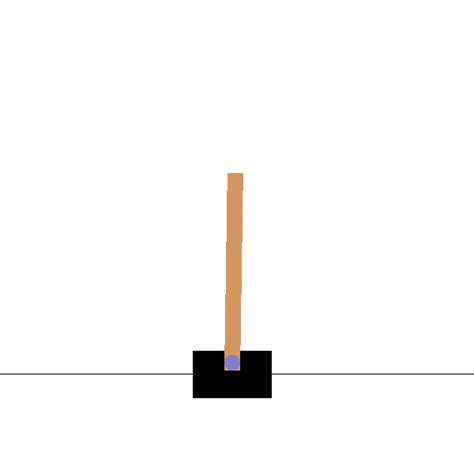
\includegraphics[width=0.7\linewidth]{img/cartpole}
	\caption[Cartpole environment]{Cartpole environment of Open-AI gym}
	\label{fig:cartpole}
\end{figure}\\
The environment state is an array of 4 values representing: (position, velocity, pole angle, and pole angular velocity). Position and angle are limited in value, while the others are not. The possible actions that can be taken are linked to a single value that can be 0 or 1, which respectively means push left or right. The reward is given by the environment for any step taken increasing the total return by 1. The conditions for which an episode is stopped are: the cartpole reaches the environment extremes, the angling pole is equal to or greater than 12° or the number of steps taken is equal to 200.\\
The goal is to reach a reward greater or equal to 175 for 100 episodes. Technically when this condition is reached the training should be stopped, but it will be extended for 1000 episodes to check the stability and convergence of the algorithm. To confront the advantage between \acrlong{nn} and \acrlong{vqa}  the trend of reward, the number of episodes taken to reach the goal, the time taken and the number of parameters will be counted.
This has been decided from the reference of other papers that used this way to benchmark classical and quantum models.
\subsubsection{Ansatz for VQA}
Different ansatz has been used for this work, the starting point was from the paper \cite{Scholik_2022} which has a corresponding Github repository that can be used for the code.
Variational circuit proposed for the paper is based from the following layer:
\begin{figure}[!h]
	\centering
	\begin{tikzpicture}
		\node(vq) {
			\begin{quantikz}
				\qw & \gate[style={fill=red!70}]{R_x(x)} & 	\gate[style={fill=cyan}]{R_y(\theta)}& \gate[style={fill=cyan}]{R_z(\theta)} & \ctrl{1} & \qw & \qw & \targ{} & \qw  \\
				\qw & \gate[style={fill=red!70}]{R_x(x)} & 	\gate[style={fill=cyan}]{R_y(\theta)}& \gate[style={fill=cyan}]{R_z(\theta)} & \targ{} & \ctrl{1} & \qw & \qw & \qw \\
				\qw & \gate[style={fill=red!70}]{R_x(x)} & 	\gate[style={fill=cyan}]{R_y(\theta)}& \gate[style={fill=cyan}]{R_z(\theta)} & \qw & \targ{} & \ctrl{1} & \qw & \qw \\
				\qw & \gate[style={fill=red!70}]{R_x(x)} & 	\gate[style={fill=cyan}]{R_y(\theta)}& \gate[style={fill=cyan}]{R_z(\theta)} & \qw & \qw & \targ{} & \ctrl{-3}  & \qw
			\end{quantikz}
		};
	\end{tikzpicture}
	\caption{Variational quantum algorithm for cartpole }
	\label{vqa dqn}
\end{figure}\\
As it can be seen, this kind of layer applies the data-reuploading approach already mentioned. This seems vital to achieve good performance concerning the classical one, for more information please consult the paper. The layer is repeated multiple times to achieve enough depth for the expressivity required to approximate the best q-value function. The measurement applied at the end uses a probabilistic approach, in fact, due to the nature of the environment a single action is required, go left or right, so to reduce the dimension output a measurement composed of two qubits corresponding to $Z \otimes Z$ is applied. After the measurement value with maximum probability is chosen and executed. To increase the performance, parameters on input and output are added, leading to the following final structure \ref{dqn hybrid}.\\
\begin{figure}[!h]
	\centering
	\resizebox {\linewidth} {!} {
		\begin{tikzpicture}
			\node[draw, label = {repeat $n$ times}](dqn) {
				\begin{quantikz}
					\qw & \gate[style={fill=red!70}]{R_x(x)} & 	\gate[style={fill=cyan}]{R_y(\theta)}& \gate[style={fill=cyan}]{R_z(\theta)} & \ctrl{1} & \qw & \qw & \targ{} & \qw   \\
					\qw & \gate[style={fill=red!70}]{R_x(x)} & 	\gate[style={fill=cyan}]{R_y(\theta)}& \gate[style={fill=cyan}]{R_z(\theta)} & \targ{} & \ctrl{1} & \qw & \qw & \qw \\
					\qw & \gate[style={fill=red!70}]{R_x(x)} & 	\gate[style={fill=cyan}]{R_y(\theta)}& \gate[style={fill=cyan}]{R_z(\theta)} & \qw & \targ{} & \ctrl{1} & \qw & \qw  \\
					\qw & \gate[style={fill=red!70}]{R_x(x)} & 	\gate[style={fill=cyan}]{R_y(\theta)}& \gate[style={fill=cyan}]{R_z(\theta)} & \qw & \qw & \targ{} & \ctrl{-3} & \qw
				\end{quantikz}
			};
			\node[right= -4mm of dqn, label = {measure}](measure) {
				\begin{quantikz}
					\qw & \gate[wires =2]{Z \otimes Z} \\
					\qw & \qw \\
					\qw & \gate[wires =2]{Z \otimes Z}\\
					\qw & \qw 
				\end{quantikz}
			};
			\node[circle, above left = -8mm and 10mm of dqn , fill=orange, label={input}] (I1) {};
			\node[circle, below = 8mm of I1 , fill=orange] (I2) {};
			\node[circle, below = 8mm of I2 , fill=orange] (I3) {};
			\node[circle, below = 8mm of I3 , fill=orange] (I4) {};
			\path (I1) edge (-4.95,1.8);
			\path (I2) edge (-4.95,0.6);
			\path (I3) edge (-4.95,-0.60);
			\path (I4) edge (-4.95,-1.8);
			\node[circle, above right = -15mm and 25mm of dqn , fill=orange, label={output}] (O1) {};
			\node[circle, below = 18mm of O1 , fill=orange] (O2) {};
			\path (6.9, 1.1) edge (O1);
			\path (6.9, -1.1) edge (O2);
		\end{tikzpicture}
	}
	\caption{Final structure for cartpole}
	\label{dqn hybrid}
\end{figure}
The original implementation used libraries Pennylane and PyTorch, this made the algorithm take around 11 hours for 5000 episodes. Due to the requirement of benchmarking the code has been rewritten using TensorFlow quantum, this allowed a speedup by reducing the time required by at least 11-12 times.
By applying multiple runs and confronting the runs made by the quantum algorithm and different kinds of neural networks this result is obtained:
\begin{figure}[!h]
	\centering
	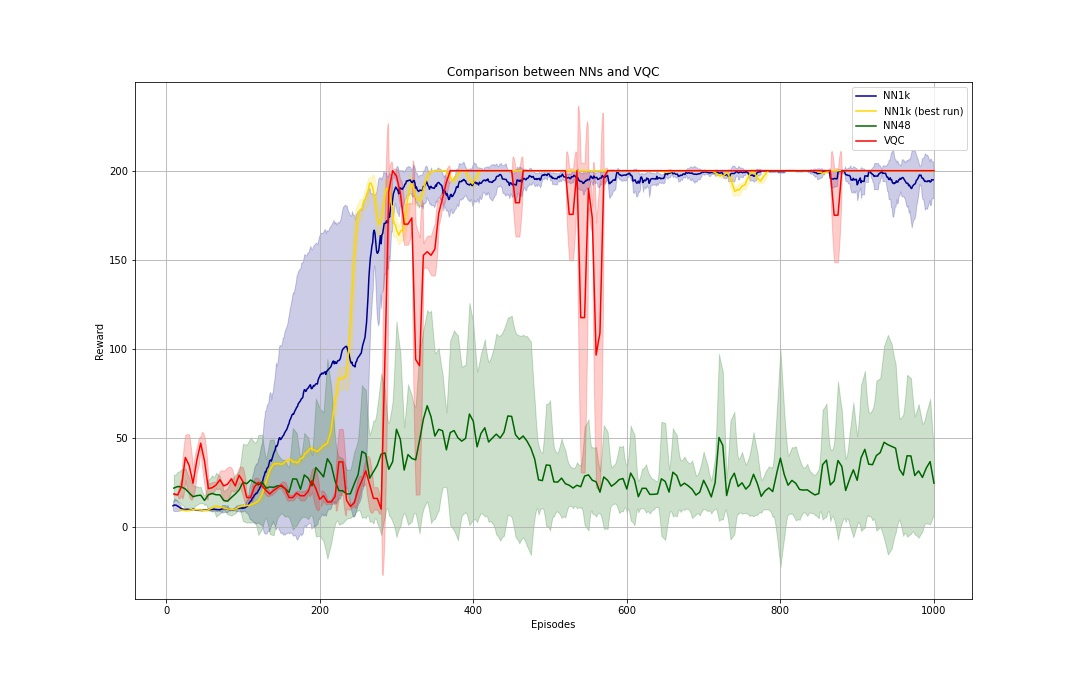
\includegraphics[width=\linewidth]{img/VQCNNcomparisonmedia}
	\caption[Benchmark of quantum and classical dqn]{In this image it has been used the mean and the variance of 10 runs of neural networks and vqa}
	\label{fig:vqcnncomparisonmedia}
\end{figure}\\
As it can be seen from the plot a neural network with the same number of vqa parameter is unable to reach the goal of cartpole and in order to have the same trend a neural network with 1256 parameters.\\
This means a quantum advantage is present in the number of parameters and expressivity of the modes with few layers. The paper referenced is more expressive and more exhaustive on all hyperparameters that have been tested, the configuration used for this benchmark is:
\begin{center}
	\begin{tabular}{|c|c|c|c|}
		\hline
		hyperparameter & NN(1256 params) & NN(48 params) & VQA \\
		\hline
		$\gamma$ & 0.99 & 0.99 & 0.99 \\
		\hline
		optimizer & Adam & Adam & Adam \\
		\hline
		batch size & 64 & 64  & 16 \\
		\hline
		learning rate & 0.001 & 0.001 & 0.01 \\
		\hline
		buffer memory & 100000 & 100000 & 10000 \\
		\hline
		$\epsilon$ start & 0.1 & 0.1 & 1 \\
		\hline
		$\epsilon$ decay & 0.99 & 0.99 & 0.99 \\
		\hline
		$\epsilon$ final & 0.001 & 0.001 & 0.01 \\
		\hline
		Loss & Smooth-L1 & Smooth-L1 & Smooth-L1 \\
		\hline
		neuron layers & (4,32)(32,32)(32,2) & (4,8)(8,2) & (4,)(2,)  \\
		\hline
		vqa layers & None & None & 5 \\
		\hline
	\end{tabular}
\end{center}
As it can be seen from the hyperparameters $\epsilon$ used for the $\epsilon$-greedy algorithm used is decreased from starting to ending value applying a formula called linear decay.\\
A better and more efficient ansatz was proposed by TensorFlow quantum exactly for this kind of problem giving to the following structure of the \acrlong{vqa}:
\begin{figure}[h]
	\centering
	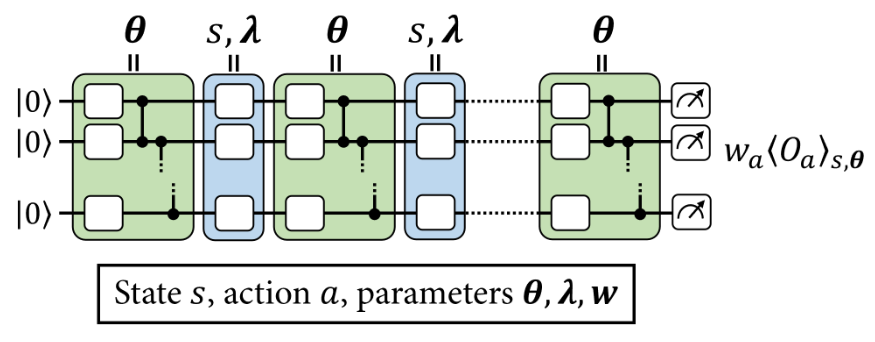
\includegraphics[width=0.8\linewidth]{img/tfq}
	\caption{Ansatz of variational circuit with data reuploading of the tensorflow quantum library}
	\label{fig:tfq}
\end{figure}\\
The differences between this kind of ansatz and \ref{dqn hybrid} are the lack of classical weights input-output and above all the encoding layer is parametrized. This means that the expressivity of this model can be tuned by finding the parameters that can give the best encoding to find afterwards the best approximation.\\
Now that the results of Cartpole have been shown proving that there can be a quantum advantage using fewer parameters, it is now changed with another environment which is based on the robotic arm and can demonstrate the quantum capabilities applied to possible future industrial applications.
\subsection{Variational quantum algorithm on robotic arm}
\subsubsection{Environment}
The previous environment is used for benchmarking and has a partial view of the capability of this algorithm. It is now time to test it on something more complex and with application in the industry: a robotic arm. \\
This technology is applied in many fields of industry such as manufacturing, cars and many others. The environment that will be used to simulate a robotic arm has been created and offered by prof. Noah Klarmann from the university of Rosenheim I would like to thank. This environment is formed of an arm composed of different links whose number can be defined, that influence both the space of state and action, with a random point which needs to be reached by the arm using its extreme.\\
The links are independent and can move in any direction with a fixed maximum velocity, which means that for every possible point that can be reached the number of steps required is not always the same. As it can be seen from this rendering:
\begin{figure}[h]
	\centering
	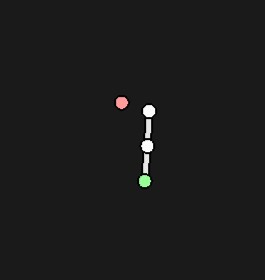
\includegraphics[width=0.45\linewidth]{img/quantum_robotic_arm_SAC_4182}
	\caption{Robotic arm with 2 links, the termination point of arm is green and the objective point is red}
	\label{fig:roboticarmsac}
\end{figure}\\
The total return is calculated for every step taken, the value is negative for every step that the arm was unable to reach the determined point and is defined as the euclidean distance between arm termination and point. If it can effectively reach the target point, a positive reward of +5 is given. The possible termination conditions are two: the steps taken are equal to 250 and the target point is reached.\\
The state tuple is composed, in the case of 2 links, as (target x, targe y, end effector x, end effector y, link angle 1, link angle 2) in the case of more links the tuple length increase adding more link angles. The action tuple has a length equal to links and in the case of 2 is : (link 1 velocity, link 2 velocities).\\
There isn't an exact condition for which the environment is considered solved, but from multiple runs and afterwards the environment rendering, it was decided to be considered solved when the mean reward was above $-40$ for the case of 2 links.
Differently from the cartpole environment, the robotic arm can be multi-discrete or continuous and for the application, it was decided to use the continuous one and use the \acrfull{sac} by substituting a complete neural network approach with a hybrid which uses the \acrshort{vqa}.
\subsubsection{Quantum SAC}
A paper has been already published which uses a quantum \acrshort{sac} approach to solve the pendulum-v0 environment, the details can be found in \cite{https://doi.org/10.48550/arxiv.2112.11921} and the pseudocode is reported in \ref{qsac}.
So from the pseudo-code, it is possible to understand that there 5 components: an actor policy, two action-value approximators and two called target action-value approximators.
The reason for which the target components must be similar to the \acrshort{dqn} case, is because usually two consecutive states are not independent and require action-values to be it to correctly update the weights an independent copy is required.
The reason for which both action and target components are double can be explained by other advances of \acrshort{dqn} which showed that using two components and taking a minimum of the two improves performance and stability.
The final component which is an actor policy, for the case of \acrshort{sac} this component will output two values: mean and variance of a gaussian distribution. From this the action will be sampled random meaning that this approach is statistical, it can be converted to deterministic by using the mean extracted from the component.\\
This policy actor in the paper is defined as a quantum-classic hybrid approach that differently from \acrshort{dqn} tries to incorporate \acrlong{nn} layers and \acrlong{vqa}. An image showing the actual structure present on the paper is \ref{fig:qsac} .\\
So of the 5 components present in this algorithm, only one uses the \acrshort{vqa} with \acrshort{nn}, this can be a limitation and afterwards, the results use an algorithm for which every component applies it. All the tests showed, are the ones with an environment that uses 2 links, this is due to a lack of time and resources. 
\begin{algorithm} \label{qsac}
	\caption{Variational Quantum Sac}
	\begin{algorithmic}
		\REQUIRE initial policy parameters $\theta$, initial action-value estimate parameters $\phi_1$ and $phi_2$, $\gamma$, $\alpha$, $\rho$, empty experience replay $D$.
		\STATE Initialize the hybrid quantum-classical policy network with $\theta$.
		\STATE Initialzie two action value networks with $\phi_1$ and $phi_2$ respectively.
		\STATE Set target-action value networks parameters: $\phi_{targ, 1} \leftarrow \phi_1$ and $\phi_{targ, 2} \leftarrow \phi_1$.
		\FOR{each time-step}
		\STATE Observe state $S$, select action $A \sim \pi_{\theta}(\cdot |S)$ and execute $A$ in the environment.
		\STATE Observe next state $S'$, reward $R$, and binary done signal $d$ to indicate whether $S'$ is terminal state or not.
		\STATE Store $(S,A,R,S',d)$ in $D$.
		\STATE Reset the environment if $d=1$.
		\STATE Sample a batch of transitions $B = {(S,A,R,S',d)}$ from $D$ randomly.
		\STATE Compute target values $y(R,S',d) = R + \gamma (1-d) (min_{i=1,2}Q_{\phi_{targ,i}} (S',A') - \alpha \log \pi_{\theta}(A',S'))$ where $A' \sim \pi(\cdot,S')$.
		\STATE Update $\phi_i$ by minimizing: $\mathbb{E}_B [(Q_{\phi_i}(S,A) - y(R,S',d))^2]$ for $i = 1,2$.
		\STATE Update $\theta$ by maximizing: $\mathbb{E}_B [min_{i=1,2} Q_{\phi_i}(S,\tilde{A}_\theta) - \alpha \log \pi_{\theta}(\tilde{A}_\theta|S)]$.
		\STATE Do a soft update for target action-value networks: $\phi_{targ,i} \leftarrow \rho \phi_{targ,i} + (1-\rho)\phi_i$ for $i=1,2$.
		\ENDFOR
	\end{algorithmic}
\end{algorithm}
\begin{figure}[H]
	\centering
	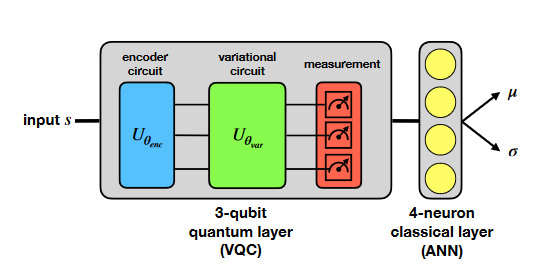
\includegraphics[width=\linewidth]{img/qsac}
	\caption{Hybirid actor policy architecture, image taken from \cite{https://doi.org/10.48550/arxiv.2112.11921}}
	\label{fig:qsac}
\end{figure}
\subsubsection{Results with hybrid actor}
Using the previous ansatz and algorithm it was decided to apply the hybrid architecture only on the actor component applying 4 and 5 layers giving a total of respectively 100 and 112 parameters.
To confront it with a \acrshort{nn} two tests were carried out using 149 and 164 parameters leading to this interesting plot. The runs could not be repeated for the lack of time and resources required, in fact, the hybrid architecture took almost 19 hours to reach this point. Even if the classical one took only 4, to benchmark them it would require at least 1 week and as it will be noticed this kind of solution is not optimal as it will be later noticed.
One of the reasons for which these runs weren't repeated multiple times is the time and resources required, in fact using multiple CPUs or applying in the future on a GPU may reduce significantly this time. Unfortunately at the time of writing, this is not possible, but it may be applied in the future.\\
Confronting results obtained using hybrid and classical components gives:  
\begin{figure}[H]
	\centering
	\includegraphics[width=\linewidth]{"img/VQA and classic actor"}
	\caption{Moving average with a time window of 30 with a mean and standard deviation of the trend.}
	\label{fig:vqa-and-classic-actor}
\end{figure}
From this an interesting fact can be noticed: all of the tests have more or less the same trend and reach the same return at around 250000 steps. As can be seen, the hybrid algorithm presents a higher steep curve confronting the classical ones and can reach the plateau slightly faster, but there isn't a clear quantum advantage due to the similar number of parameters and time steps taken.
This is quite suspicious and could mean that the critical component may not be the actor, but the critic. To confirm this suspect notice the plot of only the actor component that uses \acrlong{nn}:
\begin{figure}[H]
	\centering
	\includegraphics[width=\linewidth]{"img/classics actor"}
	\caption{Plot of the runs that uses neural netowrks for all the components.}
	\label{fig:classics-actor}
\end{figure}
As it can be noticed an increase on the number of parameters doesn't determine a great variation, instead if a plot using the hybrid algorithm and reducing the critic component size using same architecture the following plot is obtained:
\begin{figure}[H]
	\centering
	\includegraphics[width=\linewidth]{"img/VQA critic reduced"}
	\caption{Plot confronting vqa with reduced parameters of critic and previous ones.}
	\label{fig:vqa-critic-reduced}
\end{figure}
\vspace{0.5cm}
So effectively the most impacting component on the ability to reach the goal of this algorithm is not the actor, but the critic ones! Here can be found the table containing information on the structure of components where it can be noticed that except for the number of params the test runs use almost everywhere the same exact hyperparameters:
\newline
\vspace{0.2cm}
\newline
\begin{tabular}{|c|c|c|}
	\hline
	Hyperparameters & VQA 4 layers & VQA 5 layers  \\
	\hline
	$\gamma$ & 0.99 & 0.99  \\
	\hline
	$\alpha$ & 0.2 & 0.2  \\
	\hline
	learning rate & 0.0003 & 0.0003  \\
	\hline
	memory size & 1000000 & 1000000   \\
	\hline
	optimizer & Adam & Adam  \\
	\hline
	actor neurons  & (6, VQA, (1,1)) & (6, VQA, (1,1))  \\
	\hline
	actor act. func. & (linear,relu,linear) & (linear,relu,linear) \\
	\hline
	actor params & 100 & 112 \\
	\hline
	critic neurons & (8,64)(64,64)(64,1) & (8,64)(64,64)(64,1)  \\
	\hline
	critic act. func. & (linear,relu,relu,linear) & (linear,relu,relu,linear) \\
	\hline
	critic params & 4608 & 4608 \\
	\hline
	total params & 18532 & 18544 \\
	\hline
\end{tabular}
\newline
\vspace{0.5 cm}
\newline
\begin{tabular}{|c|c|c|}
	\hline
	Hyperparameters & VQA 4 layers reduced & VQA 5 layers reduced  \\
	\hline
	$\gamma$ & 0.99 & 0.99   \\
	\hline
	$\alpha$ & 0.2 & 0.2   \\
	\hline
	learning rate & 0.0003 & 0.0003   \\
	\hline
	memory size & 1000000 & 1000000   \\
	\hline
	optimizer & Adam & Adam  \\
	\hline
	actor neurons  & (6, VQA, (1,1)) & (6, VQA, (1,1))  \\
	\hline
	actor act. func. & (linear,relu,linear) & (linear,relu,linear) \\
	\hline
	actor params & 100 & 112  \\
	\hline
	critic neurons & (8,16)(16,16)(16,1) & (8,16)(16,16)(16,1)  \\
	\hline
	critic act. func. & (linear,relu,relu,linear) & (linear,relu,relu,linear) \\
	\hline
	critic params & 384 & 384\\
	\hline
	total params & 1636 & 1648\\
	\hline
\end{tabular}
\newline
\vspace{0.5 cm}
\newline
\begin{tabular}{|c|c|c|}
	\hline
	Hyperparameters & Actor NN 149 & Actor NN 164 \\
	\hline
	$\gamma$  & 0.99 & 0.99 \\
	\hline
	$\alpha$ & 0.2 & 0.2 \\
	\hline
	learning rate  & 0.0003 & 0.0003 \\
	\hline
	memory size  & 1000000 & 1000000 \\
	\hline
	optimizer  & Adam & Adam \\
	\hline
	actor neurons & (6,24,(1,1)) & (6,26,(1,1)) \\
	\hline
	actor act. func. & (linear,relu,linear) & (linear,relu,linear) \\
	\hline
	actor params & 149 & 164 \\
	\hline
	critic neurons & (8,64,64,1) & (8,64,64,1) \\
	\hline
	critic act. func. & (linear,relu,relu,linear) & (linear,relu,relu,linear) \\
	\hline
	critic params & 4608 & 4608 \\
	\hline
	total params  & 18581 & 18596 \\
	\hline
\end{tabular}\\
\\
The reason for which the total parameters are so high links to the fact that 4 critic components are required for the algorithm to work and learn.
\subsubsection{Results with hybrid actor and critic}
Now that the previous test has demonstrated that critic is the component that determines the most performance the following test will use the hybrid algorithm used for the actor and apply it to the critic. During the first tests, we noticed that the previous structure used for the actor isn't good for the critic due to maybe a high non-linearity of the map required. For this reason, the previous structure was modified by adding a hidden layer before the output to increase the expressivity of non-linearity. This is the schematic:\\
\begin{figure}[!h]
	\centering
	\resizebox {1.0\linewidth} {!} {
		\begin{tikzpicture}
			\node[draw, label = {repeat $n$ times}](vqc) {
				\begin{quantikz}
					\qw & \gate[style={fill=red!70}]{R_x(\lambda x)} & 	\gate[style={fill=cyan}]{R_y(\theta)}& \gate[style={fill=cyan}]{R_z(\theta)} & \ctrl{1} & \qw & \qw & \qw & \qw & \targ{} & \qw \\
					\qw & \gate[style={fill=red!70}]{R_x(\lambda x)} & 	\gate[style={fill=cyan}]{R_y(\theta)}& \gate[style={fill=cyan}]{R_z(\theta)} & \targ{} & \ctrl{1} & \qw & \qw & \qw & \qw & \qw \\
					\qw & \gate[style={fill=red!70}]{R_x(\lambda x)} & 	\gate[style={fill=cyan}]{R_y(\theta)}& \gate[style={fill=cyan}]{R_z(\theta)} & \qw & \targ{} & \ctrl{1} & \qw & \qw & \qw & \qw \\
					\qw & \gate[style={fill=red!70}]{R_x(\lambda x)} & 	\gate[style={fill=cyan}]{R_y(\theta)}& \gate[style={fill=cyan}]{R_z(\theta)} & \qw & \qw & \targ{} & \ctrl{1} & \qw & \qw & \qw \\
					\qw & \gate[style={fill=red!70}]{R_x(\lambda x)} & 	\gate[style={fill=cyan}]{R_y(\theta)}& \gate[style={fill=cyan}]{R_z(\theta)} & \qw & \qw & \qw & \targ{} & \ctrl{1} & \qw & \qw \\
					\qw & \gate[style={fill=red!70}]{R_x(\lambda x)} & 	\gate[style={fill=cyan}]{R_y(\theta)}& \gate[style={fill=cyan}]{R_z(\theta)} & \qw & \qw & \qw & \qw & \targ{} & \ctrl{-5} & \qw \\
				\end{quantikz}
			};
			\node[right = -4mm of vqc, label = {measure}](measure) {
				\begin{quantikz}
					\qw & \meter{} & \qw \\
					\qw & \meter{} & \qw \\
					\qw & \meter{} & \qw \\
					\qw & \meter{} & \qw \\
					\qw & \meter{} & \qw \\
					\qw & \meter{} & \qw \\
				\end{quantikz}
			};
			\node[circle, above left = -6.5mm and 10mm of vqc , fill=orange, label={input}] (I1) {};
			\node[circle, below = 8mm of I1 , fill=orange] (I2) {};
			\node[circle, below = 8mm of I2 , fill=orange] (I3) {};
			\node[circle, below = 8mm of I3 , fill=orange] (I4) {};
			\node[circle, below = 8mm of I4 , fill=orange] (I5) {};
			\node[circle, below = 8mm of I5 , fill=orange] (I6) {};
			\foreach \i in {1,2,3,4,5,6}{
				\path (I\i) edge (-5.85,3.35);
				\path (I\i) edge (-5.85,2.15);
				\path (I\i) edge (-5.85,0.95);
				\path (I\i) edge (-5.85,-0.35);
				\path (I\i) edge (-5.85,-1.55);
				\path (I\i) edge (-5.85,-2.75);
			}
			\node[circle, above right = -6.8mm and 8mm of measure , fill=orange, label={hidden}] (H1) {};
			\node[circle, below = 8mm of H1 , fill=orange] (H2) {};
			\node[circle, below = 8mm of H2 , fill=orange] (H3) {};
			\node[circle, below = 8mm of H3 , fill=orange] (H4) {};
			\node[circle, below = 8mm of H4 , fill=orange] (H5) {};
			\node[circle, below = 8mm of H5 , fill=orange] (H6) {};
			\foreach \i in {1,...,6}{
				\path (H\i) edge (7.7,3.35);
				\path (H\i) edge (7.7,2.15);
				\path (H\i) edge (7.7,0.95);
				\path (H\i) edge (7.7,-0.35);
				\path (H\i) edge (7.7,-1.55);
				\path (H\i) edge (7.7,-2.8);
			}
			\node[circle, below right = 15mm and 15mm of H2, fill=orange, label={output}] (O1) {};
			\foreach \i in {1,...,6}{
				\path (H\i) edge (O1);
			}
		\end{tikzpicture}	
	}
	\caption{Structure for critic hybrid}
	\label{critic hybrid}
\end{figure}\\
As it can be seen from the plot \ref{fig:fully_vs_partial_quantum} by converting all components to hybrid architecture it was able to have a performance very similar to the ones with the only hybrid actor. As it will be seen later this means that a smaller component that uses few parameters can reach the same performance as one with more on the Neural network. The reason for which this line is interrupted after only 250000 steps is mainly due to the high time required, in fact, to reach that step the fully hybrid algorithm took more than a week and after concluding that the algorithm was performing very similarly to the actor hybrid it was stopped.\\
\begin{figure}[H]
	\centering
	\includegraphics[width=1.0\linewidth]{"img/fully_vs_partial_quantum"}
	\caption{Comparision between only actor hybrid and all components hybrid.}
	\label{fig:fully_vs_partial_quantum}
\end{figure}
Afterwards to have a detailed cased for which multiple configurations with different sizes of the neural network were conducted to understand what kind of advantage was expected to confront the run of all-hybrid components and all neural networks. As it can be noticed from \ref{fig:all-classical-results} increasing the size of \acrlong{nn} and keeping the actor equal for all runs doesn't mean that there is an increase in performance and unfortunately, the run that uses the least number of neurons is not able to reach the objective to have a score at least -40 as average. The choice of using 21 neurons is not casual, but it has been decided to have a similar number of parameters equal to the run that uses all hybrid components.\\
\begin{figure}[H]
	\centering
	\includegraphics[width=0.95\linewidth]{"img/All classical results"}
	\caption{All classical runs with an actor component of 149 parameters}
	\label{fig:all-classical-results}
\end{figure}
\begin{figure}[H]
	\centering
	\includegraphics[width=0.95\linewidth]{"img/Best classical vs all hybrid results"}
	\caption{Plot of classical runs and all-hybrid}
	\label{fig:best-classical-vs-all-hybrid-results}
\end{figure}
So by looking at \ref{fig:best-classical-vs-all-hybrid-results}, an important result can be obtained, the all-hybrid run can reach a similar performance of all neural network components that use a higher number of neurons to reach the objective with a similar trend and time steps required. \textbf{But if the neural network model uses a similar parameter number of the all-hybrid model then it will not be able to reach the objective}. Furthermore, all the test runs have almost all the same hyperparameters for every one of them, to have a more equal confrontation of these methods. The configurations used for these runs are:
\newline
\vspace{0.2cm}
\newline
\begin{tabular}{|c|c|c|}
	\hline
	Hyperparameters & Critic hidden 21 neurons & Critic hidden 32 neurons \\
	\hline
	$\gamma$ & 0.99 & 0.99  \\
	\hline
	$\alpha$ & 0.2 & 0.2  \\
	\hline
	learning rate & 0.0003 & 0.0003  \\
	\hline
	memory size & 1000000 & 1000000   \\
	\hline
	optimizer & Adam & Adam  \\
	\hline
	actor neurons & (6,24)(24,(1,1)) & (6,24)(24,(1,1))  \\
	\hline
	actor act. func. & (linear,relu,linear) & (linear,relu,linear) \\
	\hline
	actor params & 149 & 149 \\
	\hline
	critic neurons & (8,21)(21,21)(21,1) & (8,32)(32,32)(32,1)  \\
	\hline
	critic act. func. & (linear,relu,relu,linear) & (linear,relu,relu,linear) \\
	\hline
	critic params & 651 & 1344 \\
	\hline
	total params & 2753 & 5525 \\
	\hline
\end{tabular}
\newline
\vspace{0.5 cm}
\newline
\begin{tabular}{|c|c|c|}
	\hline
	Hyperparameters & Critic hidden 64 neurons & Critic hidden 128 neurons \\
	\hline
	$\gamma$ & 0.99 & 0.99  \\
	\hline
	$\alpha$ & 0.2 & 0.2  \\
	\hline
	learning rate & 0.0003 & 0.0003  \\
	\hline
	memory size & 1000000 & 1000000   \\
	\hline
	optimizer & Adam & Adam  \\
	\hline
	actor neurons & (6,24)(24,(1,1)) & (6,24)(24,(1,1))  \\
	\hline
	actor act. func. & (linear,relu,linear) & (linear,relu,linear) \\
	\hline
	actor params & 149 & 149 \\
	\hline
	critic neurons & (8,64)(64,64)(64,1) & (8,128)(128,128)(128,1)  \\
	\hline
	critic act. func. & (linear,relu,relu,linear) & (linear,relu,relu,linear) \\
	\hline
	critic params & 4672 & 17536 \\
	\hline
	total params & 18837 & 70293 \\
	\hline
\end{tabular}
\newline
\vspace{0.5 cm}
\newline
\begin{tabular}{|c|c|c|}
	\hline
	Hyperparameters & Critic hidden 256 neurons & All hybrid \\
	\hline
	$\gamma$ & 0.99 & 0.99  \\
	\hline
	$\alpha$ & 0.2 & 0.2  \\
	\hline
	learning rate & 0.0003 & 0.0003  \\
	\hline
	memory size & 1000000 & 1000000   \\
	\hline
	optimizer & Adam & Adam  \\
	\hline
	actor neurons & (6,24)(24,(1,1)) & (6,VQA(5 layers),(1,1))  \\
	\hline
	actor act. func. & (linear,relu,linear) & (linear,relu,linear) \\
	\hline
	actor params & 149 & 112 \\
	\hline
	critic neurons & (8,256)(256,256)(256,1) & (8,VQA(20 layers),8,1)  \\
	\hline
	critic act. func. & (linear,relu,relu,linear) & (linear,relu,relu,linear) \\
	\hline
	critic params & 67840 & 650 \\
	\hline
	total params & 271.509 & 2712 \\
	\hline
\end{tabular}
\newline
\vspace{0.2 cm}
\newline
Focusing on the number of parameters and the previous plots a conclusion can be extrapolated: to have similar trends between the hybrid model and neural networks, which are the ones with 64 neurons for hidden layers or more, it is required to have at least 7 times the number of parameters!. In fact from the previous table hybrid model uses around 2700 parameters, while the neural network with 64 uses 19000. Furthermore, as it can be seen from plot \ref{fig:best-classical-vs-all-hybrid-results} even the biggest neural network is not always able to follow the trend of the hybrid and reach the objective with the same number of steps and notice that uses around 100 times the parameters of hybrid.